% Ensure that you compile using XeLaTeX !!! PDFTex has problems with some of the packages used
\documentclass[12pt]{article}
\setlength\parindent{0pt}

\usepackage{parskip}
\usepackage[margin=0.5in]{geometry}
\usepackage{fullpage}
\usepackage{moresize}
\usepackage{graphicx}
\usepackage{caption}
\usepackage{subcaption}
\usepackage{float}
\usepackage{xcolor}
\usepackage{soul}
\usepackage{fontspec}
\setmainfont{Doulos SIL}

\begin{document}

\begin{center}
\textbf{{\color{violet}{\HUGE 20201117 Tuesday\\}}}

\textbf{{\color{violet}{\HUGE ALL EXAMS (with notes)\\}}}

\end{center}
\newpage

\begin{center}
\textbf{{\color{blue}{\HUGE START OF EXAM\\}}}

\textbf{{\color{blue}{\HUGE Student ID: 42792\\}}}

\textbf{{\color{blue}{\HUGE 4:00\\}}}

\end{center}
\newpage

{\large Question 1}\\

Topic: Transcription\\
Source: Week 2 Handout, Part II\\

Is this a reasonable transcription of this word? Explain why.\\

<mine>: {[mɑɪn]}


~\\
INSTRUCTOR NOTES: yes


\vfill
Excellent (3) ~~~ Good (2.2) ~~~ Fair (1.7) ~~~ Poor (0)
\newpage

{\large Question 2}\\

Topic: Phonological Features\\
Source: Homework 2, Question 1\\

Explain which sound should be removed to make this a natural class (assuming SNAE, except that there are no diphthongs, no [ə] or [ʌ], no syllabic consonants, and no [w̥]), and what the minimum set of features would be to describe the resulting natural class.\\

{[i]}, {[ɪ]}, {[e]}, {[ɛ]}, {[æ]}, {[ɑ]}, {[ɔ]}, {[o]}, {[ʊ]}, {[u]}, {[ʒ]}, {[k]}, {[ɡ]}, {[ŋ]}, {[w]}


~\\
INSTRUCTOR NOTES: [ʒ] should be removed, so that we have the natural class of dorsal segments; this could be minimally represented with [DORSAL]


\vfill
Excellent (3) ~~~ Good (2.2) ~~~ Fair (1.7) ~~~ Poor (0)
\newpage

\begin{center}
\textbf{{\color{red}{\HUGE END OF EXAM}}}\\

\end{center}
\newpage

\begin{center}
\textbf{{\color{blue}{\HUGE START OF EXAM\\}}}

\textbf{{\color{blue}{\HUGE Student ID: 94549\\}}}

\textbf{{\color{blue}{\HUGE 4:10\\}}}

\end{center}
\newpage

{\large Question 1}\\

Topic: Skewed Distributions\\
Source: Week 5 Handout, Question 6\\

If I gave you a new word in Malto, [di\_\_u], would it be possible to predict whether it's [d] or [t] that goes in the blank? Explain why or why not.\\

\begin{figure}[H]
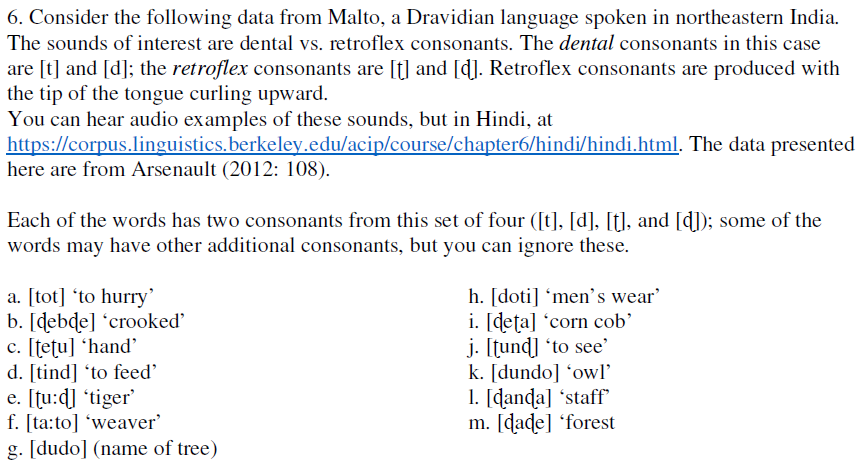
\includegraphics{../images/malto.png}
\end{figure}

~\\
INSTRUCTOR NOTES: No, it's not possible. In Malto, you can predict that there are two dental or two retroflex stops in a word, but you can't predict the voicing. These two sounds are both dental, so there's no way to predict.


\vfill
Excellent (3) ~~~ Good (2.2) ~~~ Fair (1.7) ~~~ Poor (0)
\newpage

{\large Question 2}\\

Topic: Other (pre-midterm)\\
Source: Week 4 Handout, Part II, Question 2(iii)\\

Explain how you would figure out the meaning of this Swahili word. (To be clear: you do NOT need to give me the meaning itself -- just explain the process of figuring it out.)\\

{[tunampenda]}

\begin{figure}[H]
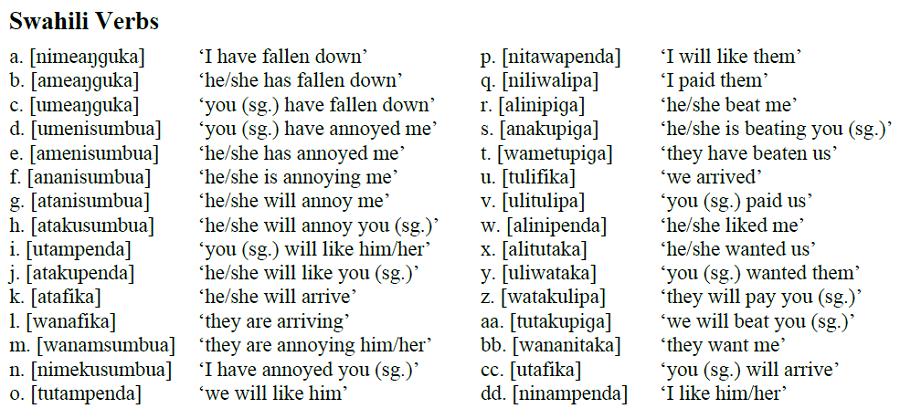
\includegraphics{../images/swahiliverbs.png}
\end{figure}

~\\
INSTRUCTOR NOTES: (we like him/her)


\vfill
Excellent (3) ~~~ Good (2.2) ~~~ Fair (1.7) ~~~ Poor (0)
\newpage

\begin{center}
\textbf{{\color{red}{\HUGE END OF EXAM}}}\\

\end{center}
\newpage

\begin{center}
\textbf{{\color{blue}{\HUGE START OF EXAM\\}}}

\textbf{{\color{blue}{\HUGE Student ID: 59669\\}}}

\textbf{{\color{blue}{\HUGE 4:20\\}}}

\end{center}
\newpage

{\large Question 1}\\

Topic: Articulatory Phonetics\\
Source: Week 3 Handout, Question 3\\

Explain why the additional vowel below either does or does not belong in the phonetic natural class defined by the original set of SNAE vowels.\\

Original set: {[æ]}, {[ɑ]}

Addition: {[ɑʊ]}


~\\
INSTRUCTOR NOTES: should recognize that there's more than one vowel sound, which makes it somewhat difficult to categorize; best answers will say that the diphthong is crucially a diphthong and so can't also go in this class


\vfill
Excellent (3) ~~~ Good (2.2) ~~~ Fair (1.7) ~~~ Poor (0)
\newpage

{\large Question 2}\\

Topic: Other (pre-midterm)\\
Source: Week 4 Handout, Part II, Question 3\\

Explain how you would figure out what the Luiseño form is for the morpheme whose meaning is given below. (To be clear: you do NOT need to give me the form itself -- just explain the process of figuring it out.)\\

‘drink’

\begin{figure}[H]
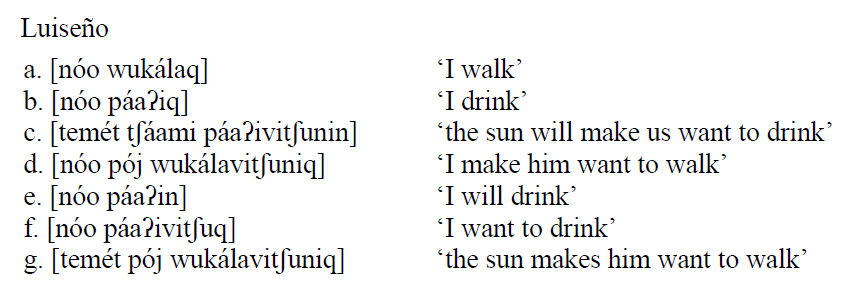
\includegraphics{../images/luiseno.png}
\end{figure}

~\\
INSTRUCTOR NOTES: ([páaʔi])


\vfill
Excellent (3) ~~~ Good (2.2) ~~~ Fair (1.7) ~~~ Poor (0)
\newpage

\begin{center}
\textbf{{\color{red}{\HUGE END OF EXAM}}}\\

\end{center}
\newpage

\begin{center}
\textbf{{\color{blue}{\HUGE START OF EXAM\\}}}

\textbf{{\color{blue}{\HUGE Student ID: 67125\\}}}

\textbf{{\color{blue}{\HUGE 4:30\\}}}

\end{center}
\newpage

{\large Question 1}\\

Topic: Phonological Features\\
Source: Homework 2, Question 1\\

Explain which sound should be removed to make this a natural class (assuming SNAE, except that there are no diphthongs, no [ə] or [ʌ], no syllabic consonants, and no [w̥]), and what the minimum set of features would be to describe the resulting natural class.\\

{[i]}, {[ɪ]}, {[e]}, {[ɛ]}, {[æ]}, {[ɑ]}, {[ɔ]}, {[o]}, {[ʊ]}, {[u]}, {[ʒ]}, {[k]}, {[ɡ]}, {[ŋ]}, {[w]}


~\\
INSTRUCTOR NOTES: [ʒ] should be removed, so that we have the natural class of dorsal segments; this could be minimally represented with [DORSAL]


\vfill
Excellent (3) ~~~ Good (2.2) ~~~ Fair (1.7) ~~~ Poor (0)
\newpage

{\large Question 2}\\

Topic: Articulatory Phonetics\\
Source: Homework 1, Question 3(a)\\

Could this image be the result of producing the sound represented by the given IPA symbol? Why or why not?\\

{[t͡ʃ]}

\begin{figure}[H]
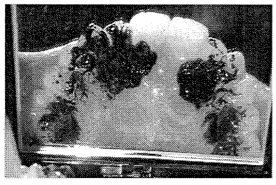
\includegraphics{../images/staticpalatography_fricative.png}
\end{figure}

~\\
INSTRUCTOR NOTES: no


\vfill
Excellent (3) ~~~ Good (2.2) ~~~ Fair (1.7) ~~~ Poor (0)
\newpage

\begin{center}
\textbf{{\color{red}{\HUGE END OF EXAM}}}\\

\end{center}
\newpage

\begin{center}
\textbf{{\color{blue}{\HUGE START OF EXAM\\}}}

\textbf{{\color{blue}{\HUGE Student ID: 96220\\}}}

\textbf{{\color{blue}{\HUGE 4:40\\}}}

\end{center}
\newpage

{\large Question 1}\\

Topic: Articulatory Phonetics\\
Source: Homework 1, Question 3(a)\\

Could this image be the result of producing the sound represented by the given IPA symbol? Why or why not?\\

{[ɾ]}

\begin{figure}[H]
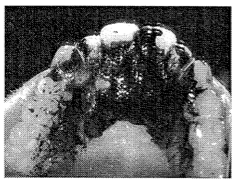
\includegraphics{../images/staticpalatography_stop.png}
\end{figure}

~\\
INSTRUCTOR NOTES: yes


\vfill
Excellent (3) ~~~ Good (2.2) ~~~ Fair (1.7) ~~~ Poor (0)
\newpage

{\large Question 2}\\

Topic: Other (pre-midterm)\\
Source: Week 4 Handout, Part II, Question 3\\

Explain how you would figure out what the Luiseño form is for the morpheme whose meaning is given below. (To be clear: you do NOT need to give me the form itself -- just explain the process of figuring it out.)\\

‘third person masc. object’ (‘him’)

\begin{figure}[H]
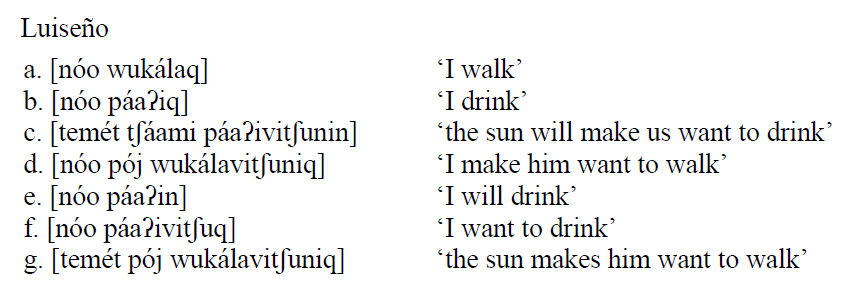
\includegraphics{../images/luiseno.png}
\end{figure}

~\\
INSTRUCTOR NOTES: ([pój])


\vfill
Excellent (3) ~~~ Good (2.2) ~~~ Fair (1.7) ~~~ Poor (0)
\newpage

\begin{center}
\textbf{{\color{red}{\HUGE END OF EXAM}}}\\

\end{center}
\newpage

\begin{center}
\textbf{{\color{blue}{\HUGE START OF EXAM\\}}}

\textbf{{\color{blue}{\HUGE Student ID: 16922\\}}}

\textbf{{\color{blue}{\HUGE 4:50\\}}}

\end{center}
\newpage

{\large Question 1}\\

Topic: Acoustics\\
Source: Week 9 Handout, Question 7\\

Explain why each numbered, underlined statement is true or false. If it is false, explain one way that you could correct it.\\

Sound is an invisible phenomenon. Sound can travel through any substance, $^1$\ul{such as a liquid, solid, or a gas.} $^2$\ul{It involves the transfer of the matter in that substance} from one place to another.\\\\Sound is a particular kind of wave known as $^3$\ul{a compression wave}. $^4$\ul{When the molecules are really close together, we say they are ``rarefied'' and when they are really far apart, we say they are ``compressed.''}


~\\
INSTRUCTOR NOTES: 1 - true.\\2 - false (it involves the transfer of energy... or anything about the matter itself not moving but only vibrating, etc). \\3 - true.\\4 - false (when the molecules are really close together, we say they are compressed and when the molecules are really far apart, we say they are rarefied).


\vfill
Excellent (3) ~~~ Good (2.2) ~~~ Fair (1.7) ~~~ Poor (0)
\newpage

{\large Question 2}\\

Topic: Other (pre-midterm)\\
Source: Week 5 \& 6 Handouts\\

Explain how you could analyze this dataset in terms of sequential patterns vs. paradigmatic patterns.\\

\begin{figure}[H]
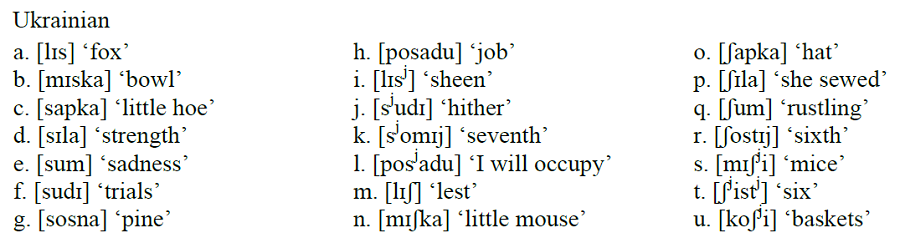
\includegraphics{../images/ukrainian.png}
\end{figure}

~\\
INSTRUCTOR NOTES: 


\vfill
Excellent (3) ~~~ Good (2.2) ~~~ Fair (1.7) ~~~ Poor (0)
\newpage

\begin{center}
\textbf{{\color{red}{\HUGE END OF EXAM}}}\\

\end{center}
\newpage

\end{document}

